
\appendix
\section{Three-party NFT exchange cycle}
Another example is a three-party exchange cycle. Each party uses ephemeral resource logics to express their intents.
\hfill\break
\hfill\break
\textbf{Step 1:} specify intents

\begin{itemize}
    \item \textbf{Alice's intent:} Alice wants to exchange her star NFT resource $R^A_{star}$ for a blue dolphin NFT resource $R_{dolphin}$
    \item \textbf{Bob's intent:} Bob wants to exchange his blue dolphin NFT $R^B_{dolphin}$ for a tree NFT resource $R_{tree}$
    \item \textbf{Charlie's intent:} Charlie wants to exchange his tree NFT $R^C_{tree}$ for a star NFT resource $R_{star}$
\end{itemize}

\begin{center}
    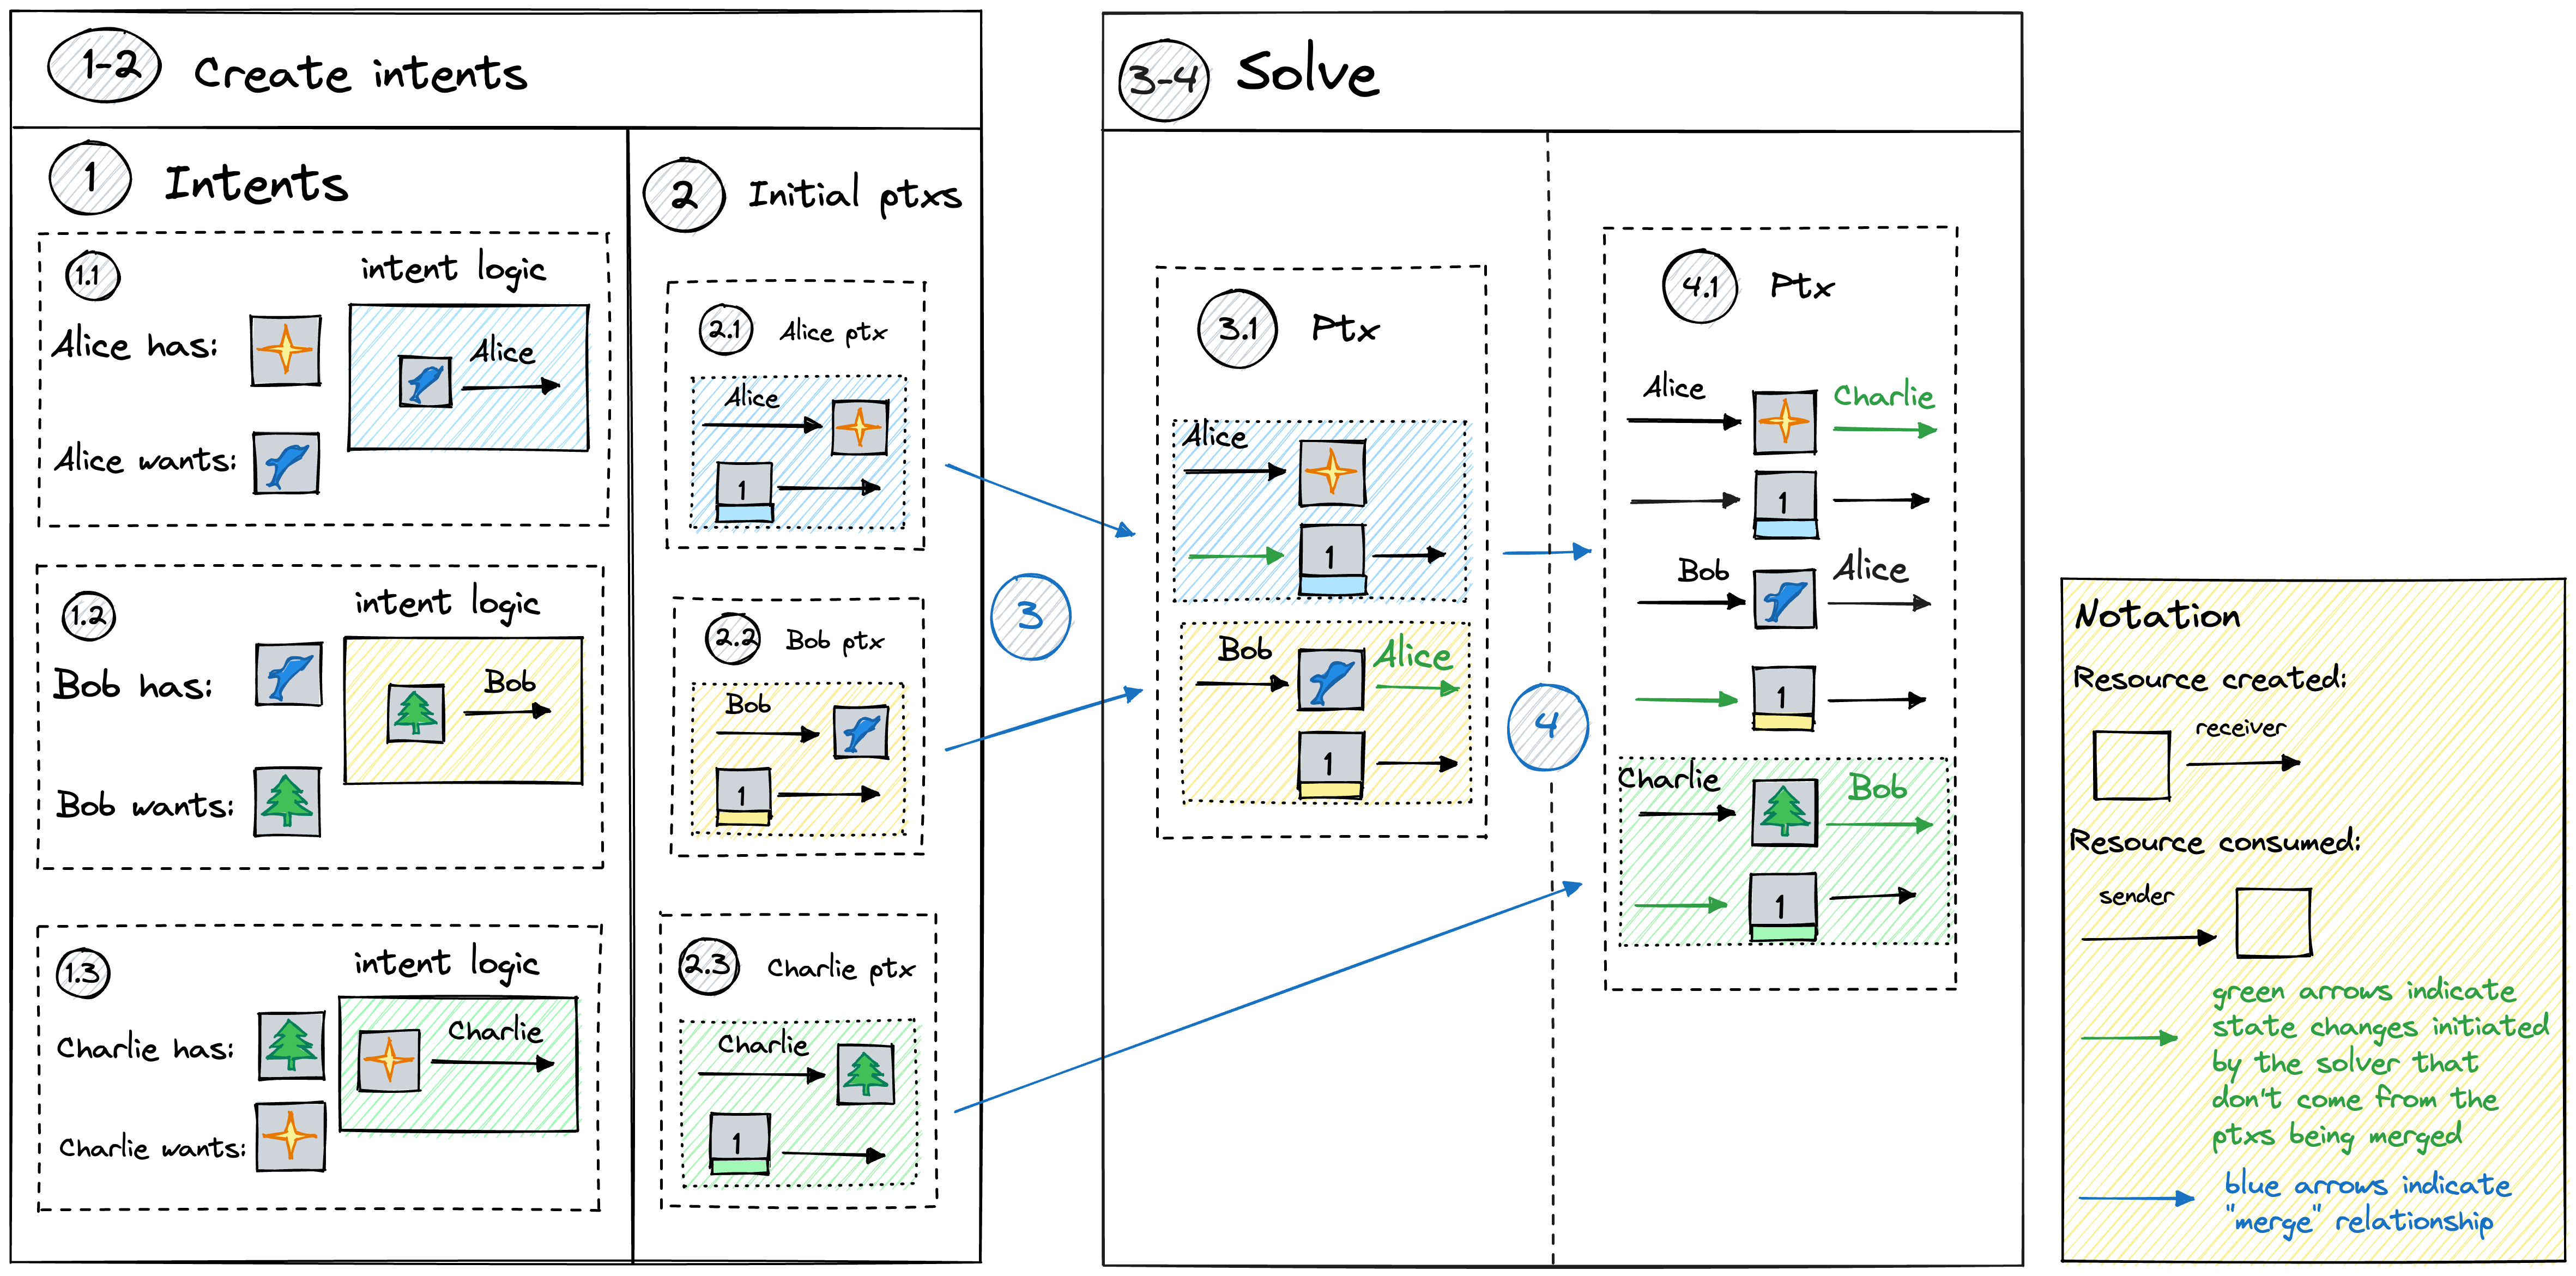
\includegraphics[width = \textwidth]{3party_rm_new.png}
\end{center}

\textbf{Step 2:} create initial transactions

Alice's initial transaction:
\begin{itemize}
    \item $rts= \{rt_{R^A_{star}}\}$
    \item $cms = \{cm_{R^A_{I^{A}}}\}$
    \item $nfs = \{nf_{R^A_{star}}\}$
    \item Proofs:
    \begin{itemize}
        \item $\Pi^A_{\Delta}$
        \item $\Pi^A_{compl}$
        \item $\Pi^A_{rl} = \{\pi^A_{star}, \pi^A_I\}$
    \end{itemize}
    \item $\Delta \mapsto \{I^{A}: 1, star: -1, \}$ – for simplicity, represent $\Delta$ as a dictionary
    \item $extra = extra^A$
    \item $\Phi = \Phi^A$
\end{itemize}

Bob's initial transaction:
\begin{itemize}
    \item $rts = \{rt_{R^B_{dolphin}}\}$
    \item $cms = \{cm_{R^B_{I^{B}}}\}$
    \item $nfs = \{nf_{R^B_{doplhin}}\}$
    \item Proofs:
    \begin{itemize}
        \item $\Pi^B_{\Delta}$
        \item $\Pi^B_{compl}$
        \item $\Pi^B_{rl} = \{\pi^B_{dolphin}, \pi^B_I\}$
    \end{itemize}
    \item $\Delta \mapsto \{I^{B}: 1, dolphin: -1 \}$
    \item $extra = extra^B$
    \item $\Phi = \Phi^B$
\end{itemize}

Charlie's initial transaction:
\begin{itemize}
    \item $rts = \{rt_{R^C_{tree}}\}$
    \item $cms = \{cm_{R^C_{I^{C}}}\}$
    \item $nfs = \{nf_{R^C_{tree}}\}$
    \item Proofs:
    \begin{itemize}
        \item $\Pi^C_{\Delta}$
        \item $\Pi^C_{compl}$
        \item $\Pi^C_{rl} = \{\pi^C_{tree}, \pi^C_I\}$
    \end{itemize}
    \item $\Delta \mapsto \{I^{C}: 1, tree: -1, \}$
    \item $extra = extra^C$
    \item $\Phi = \Phi^C$
\end{itemize}

\textbf{Step 3:} solve

A solver $S_1$, seeing $TX^A$ and $TX^B$, creates a transaction $TX^{S_1}$ (on the diagram: $TX_{3.1}$, green arrows):

\begin{itemize}
    \item $rts = \{rt_{R^A_{I^{A}}}\}$
    \item $cms = \{cm_{R^A_{dolphin}}\}$
    \item $nfs = \{nf_{R^A_{I^{A}}}\}$
        \item Proofs:
    \begin{itemize}
        \item $\Pi^{S_1}_{\Delta}$
        \item $\Pi^{S_1}_{compl}$
        \item $\Pi^{S_1}_{rl} = \{\pi^{S_1}_{dolphin}, \pi^{S_1}_{I_A}\}$
    \end{itemize}
    \item $\Delta \mapsto \{dolphin: 1, I^{A}: -1\}$
    \item $extra = extra^{S_1}$
    \item $\Phi = \Phi^{S_1}$
\end{itemize}

and composes all three transactions together, producing a transaction $TX_{3.1}$:

\begin{itemize}
    \item $rts = \{rt_{R^A_{star}}, rt_{R^B_{dolphin}}, rt_{R^A_{I^{A}}}\}$
    \item $cms = cms^{A} \sqcup cms^B \sqcup cms^{S_1} =\{
    cm_{R^A_{I^{A}}}, cm_{R^B_{I^{B}}}, cm_{R^A_{dolphin}}\}$
    \item $nfs = nfs^A \sqcup nfs^B \sqcup nfs^{S_1} = \{nf_{R^A_{star}}, nf_{R^B_{dolphin}}, nf_{R^A_{I^{A}}}\}$
        \item Proofs:
    \begin{itemize}
        \item $\Pi^{3.1}_{\Delta} = AGG(\Pi^A_{\Delta}, \Pi^B_{\Delta}, \Pi^{S_1}_{\Delta})$
        \item $\Pi^{3.1}_{compl} = \Pi^A_{compl} \sqcup \Pi^B_{compl} \sqcup \Pi^{S_1}_{compl}$
        \item $\Pi^{3.1}_{rl} = \Pi^A_{rl} \sqcup \Pi^B_{rl} \sqcup \Pi^{S_1}_{rl}$
    \end{itemize}
    \item $\Delta \mapsto \{I^{A}: 0, I^{B}: 1, star: -1, dolphin: 0\}$
    \item $extra = extra^A \cup extra^B \cup extra^{S_1}$
    \item $\Phi = G(\Phi^A, \Phi^B, \Phi^{S_1})$
\end{itemize}

\textbf{Step 4:} continue solving

Seeing $TX^C$ and $TX_{3.1}$, a solver $S_2$ creates a transaction $TX_{S_2}$ (on the diagram: $TX_{4.1}$, green arrows):

\begin{itemize}
    \item $rts = \{rt_{R^C_{I^{C}}}, rt_{R^B_{I^{B}}}\}$
    \item $cms = \{
    cm_{R^C_{star}}, cm_{R^B_{tree}}\}$
    \item $nfs = \{nf_{R^C_{I^{C}}}, nf_{R^B_{I^{B}}}\}$
    \item Proofs:
    \begin{itemize}
        \item $\Pi^{S_2}_{\Delta}$
        \item $\Pi^{S_2}_{compl}$
        \item $\Pi^{S_2}_{rl} = \{\pi^{S_2}_{star}, \pi^{S_2}_{I_C}\, \pi^{S_2}_{tree}, \pi^{S_2}_{I_B}\}$
    \end{itemize}
    \item $\Delta \mapsto \{I^{C}: -1, I^{B}: -1, star: 1, tree: 1\}$
    \item $extra = extra^{S_2}$
    \item $\Phi = \Phi^{S_2}$
\end{itemize}

and composes all three into a balanced transaction $TX_{4.1}$:

\begin{itemize}
    \item $rts = \{rt_{R^A_{star}}, rt_{R^B_{dolphin}}, rt_{R^C_{tree}}, rt_{R^A_{I^{A}}}, rt_{R^B_{I^{B}}}, rt_{R^C_{I^{C}}}\}$
    \item $cms = cms^{TX^{3.1}} \sqcup cms^{S_2} =\{cm_{R^A_{dolphin}}, cm_{R^B_{tree}}, cm_{R^C_{star}}, cm_{R^A_{I^{A}}}, cm_{R^B_{I^{B}}}, cm_{R^C_{I^{C}}}\}$
    \item $nfs = nfs^{TX^{3.1}} \sqcup nfs^{S_2} = \{nf_{R^A_{star}}, nf_{R^B_{dolphin}}, nf_{R^C_{tree}}, nf_{R^A_{I^{A}}}, nf_{R^B_{I^{B}}}, nf_{R^C_{I^{C}}}\}$
    \item Proofs:
    \begin{itemize}
        \item $\Pi^{4.1}_{\Delta} = AGG(\Pi^{3.1}_{\Delta}, \Pi^{C}_{\Delta}, \Pi^{S_2}_{\Delta})$
        \item $\Pi^{4.1}_{compl} = \Pi^C_{compl} \sqcup \Pi^{3.1}_{compl} \sqcup \Pi^{S_2}_{compl}$
        \item $\Pi^{4.1}_{rl} = \Pi^C_{rl} \sqcup \Pi^{3.1}_{rl} \sqcup \Pi^{S_2}_{rl}$
    \end{itemize}
    \item $\Delta \mapsto \{I^{A}: 0, I^{B}: 0, I^{C}: 0, star: 0, dolphin: 0, tree: 0\}$
    \item $extra = extra^A \cup extra^B \cup extra^C \cup extra^{S_1} \cup extra^{S_2}$
    \item $\Phi = G(\Phi^A, \Phi^B, \Phi^{S_1}, \Phi^C, \Phi^{S_2})$
\end{itemize}

In practice, the step of creation of the transactions $TX_{S_1}$ and $TX_{S_2}$ can be merged with the composing step, but we separate the steps for clarity.
